\section{Implementación de atractor Determinístico - Estocástico}

\subsection{Introduction}

En los últimos treinta años, los sistemas caóticos han producido una revolución en nuestra visión de la naturaleza ya que tienen dos características contrastantes:
(1) son deterministas porque un modelo matemático determina su dinámica, pero
(2) debido a su sensibilidad a las condiciones iniciales, se pierde la predicción a largo plazo y, en consecuencia, pueden incluirse en la clase de sistemas estocásticos que se estudian mediante herramientas estadísticas.
En realidad, si los sistemas caóticos pudieran implementarse con una precisión infinita, serían deterministas en sentido estricto, pero la precisión infinita es un ideal imposible de alcanzar en la electrónica digital.

Esta \emph{dualidad determinista-estocástica} hace que los sistemas caóticos sean especialmente interesantes para las aplicaciones de ingeniería, en la medida en que las señales generadas pueden usarse como ruidos controlados en una amplia gama de aplicaciones.
Sin embargo, las secuencias caóticas realmente presentan correlaciones internas no lineales, lo que las hace inadecuadas para ser utilizadas como "buenas" PRNG.
Es necesario utilizar técnicas de aleatorización para mejorar la aleatoriedad de la serie \cite{DeMicco2008}.

En aplicaciones digitales, el tiempo y la variable de estado tienen valores discretos.
La discretización de tiempo impone el uso de un algoritmo para aproximar las ecuaciones diferenciales de tiempo continuo que modelan el sistema.
El algoritmo más simple es el método de Euler de primer orden en el que los diferenciales se reemplazan directamente por incrementos finitos.
Los algoritmos más elaborados, como los algoritmos de paso variable Runge-Kutta de cuarto orden (o superior), hacen que el sistema discreto evolucione más cerca del sistema continuo, pero con mayores requisitos de recursos de hardware y tiempos de cálculo.
En consecuencia, deben usarse solo si la exactitud es un requisito de la aplicación específica.
Este no es el caso en PRNG, donde la aleatoriedad es la característica principal que debe garantizarse.

Para hacer los cálculos aritméticos, las computadoras deben representar internamente las señales por un número finito de bits, esto significa que los valores se describen usando aritmética de precisión finita.
Esta restricción puede ser crítica para un sistema caótico ya que es extremadamente sensible a la aritmética empleada e incluso puede perder su comportamiento caótico.

En este capítulo, implementamos un oscilador discreto de Lorenz obtenido mediante el uso del algoritmo de primer orden de Euler y tres estándares de representación diferentes.
Además aplicamos técnicas de aleatorización a las variables de estado para obtener un PRNG en tiempo real.
El objetivo de este trabajo es estudiar la influencia del procedimiento de discretización en la dinámica del sistema.
En \cite{DeMicco2010} se estudió el grado de estocasticidad de un sistema caótico determinista mediante su implementación en coma flotante de precisión simple (32 bits).

La determinación del grado de estocasticidad tiene como objetivo proporcionar una metodología de diseño optimizada para la utilidad prevista dada al sistema caótico.
Así, por ejemplo, hay aplicaciones que requieren que el sistema caótico reemplace un sistema estocástico (criptografía \cite{Fernandez2003}, generadores de secuencia para difundir comunicaciones de espectro \cite{Setti2004, DeMicco2007B}, generadores de números pseudoaleatorios \cite{Kocarev2003, Larrondo2006, DeMicco2009}, reducción de la interferencia electromagnética \cite{Callegari2003A}, etc.).
Por otro lado, algunas aplicaciones requieren previsibilidad a largo plazo, por ejemplo para reproducir el sistema caótico de la manera más precisa posible, este es el caso de las comunicaciones analógicas que usan portadores de sincronización caóticos \cite{Kocarev1995, Hidalgo2001}.

Otro problema es la determinación exacta del período de la secuencia pseudoaleatoria.
Para generadores que se basan en operaciones lineales, el problema se ha estudiado en profundidad y existen criterios de diseño bien conocidos para obtener dispositivos de ciclo máximo.
Ejemplos de algoritmos lineales son: el algoritmo Mersenne Twister que es un generador de números aleatorios muy rápido de período $T = 2^{19937} - 1$ \cite{Matsumoto1998} y Multiply-With-Carry (MWC), un método inventado por George Marsaglia para la generación de secuencias de enteros aleatorios basados en un conjunto inicial de dos a muchos miles de valores de semilla elegidos al azar, presenta períodos inmensos, que van desde alrededor de $2 ^ {60}$ a $2 ^ {2000000}$ \cite{Marsaglia1991}.
Sin embargo, desde el punto de vista criptográfico son débiles.
Cuando se trata de aplicaciones criptográficas, no se recomiendan métodos lineales para generar secuencias pseudoaleatorias (como LFSR, LCG o sus combinaciones adecuadas), ya que algoritmos eficientes para predecir la secuencia sobre la base de una secuencia de observación relativamente corta están a disposición \cite{Boyar1989, Plumstead1982}.
Por otro lado, para la mayoría de las familias de generadores no lineales, el problema parece ser intratable y, con pocas excepciones, no suele existir una evaluación analítica de sus períodos \cite{kocarev2011}.

Elegimos el sistema caótico de Lorenz porque es un sistema ampliamente estudiado y también ha sido implementado por otros autores con diferentes metodologías \cite{Asseri2002, Azzaz2009, Azzaz2010}.
Por ejemplo, en \cite{Asseri2002}, se implementó un oscilador caótico Lorenz mediante una toolbox del Generador de Sistemas Xilinx que funciona bajo \textit{MATLAB-Simulink\textsuperscript{\copyright}}.
Esta toolbox convierte el modelo MATLAB-Simulink en el modelo de Xilinx System Generator.
Luego se obtiene el código VHDL.
Como es una operación automática, no permite ciertos cambios específicos y presenta algunas limitaciones.
La operación de integración se aproximó con el algoritmo de Euler, utilizando bloques de suma y retardo.
La implementación propuesta en \cite{Azzaz2009} y \cite{Azzaz2010} usa $RK4$ en una arquitectura de punto fijo de $32$ bits.

En esta sección se utilizó el software \textit{QuartusII\textsuperscript{\copyright} 7.2} para generar el lenguaje de descripción de hardware VHDL y la implementación física se realiza en la placa de desarrollo \textit{Altera\textsuperscript{\copyright} Cyclone III EP3C12}.
Tres representaciones numéricas son estudiadas:
1) punto flotante IEEE 754 estándar,
2) punto fijo decimal, y
3) aritmética entera \cite{Gonzalez2003}.
Cada representación implica una cantidad diferente de bits.
Consideramos dos representaciones de coma flotante para los estándares simple o doble, con $32$ y $64$ bits respectivamente para representar el signo, el exponente y la mantisa;
La aritmética decimal de punto fijo usa $p$ bits para representar la parte entera y $m$ bits para representar la parte fraccional.
Consideramos representaciones de punto fijo de $32$ y $64$ bits con $9$ bits para la parte entera y $1$ bit para el signo y los $22$ o $54$ bits restantes para la parte fraccionaria.
En los aritméticos enteros $k$ bits el alfabeto tiene $2^k$ símbolos.
Consideramos $k=54$.

Para cuantificar la aleatoriedad del sistema, se utiliza el conjunto de pruebas DIEHARD de Marsaglia.
Estas pruebas han sido ampliamente utilizadas en la literatura abierta y son muy efectivas para clasificar sistemas determinísticos y estocásticos.

\subsection{Discretización temporal del oscilador de Lorenz}
\label{sec:lorenzdigit}

El sistema de Lorenz se define mediante el siguiente conjunto de ecuaciones diferenciales ordinarias acopladas:
%
\begin{eqnarray} \label{eq:lorconti}
\frac{dx}{dt}&=&-\delta(x-y) \ , \nonumber \\
\frac{dy}{dt}&=&\Gamma x-y-xz \ , \\
\frac{dz}{dt}&=&-bz+xy \ , \nonumber
\end{eqnarray}
%
donde $\delta$, $\Gamma$ y $b$ son parámetros constructivos del sistema.
Para ciertos valores de estos parámetros, el sistema tiene un comportamiento caótico.
Siempre se requiere un algoritmo para convertir un sistema dinámico continuo en un sistema dinámico de tiempo discreto.
El algoritmo más simple fue propuesto por Euler y, para las Ecs. \ref{eq:lorconti} surge el siguiente modelo discreto:
%
\begin{eqnarray}\label{eq:loreuler}
{\widetilde X}_{t+\Delta t}&=&{\widetilde X}_{t}+ \Delta t \left[
- \delta \left( {\widetilde X}_{t}-{\widetilde Y}_{t} \right)
\right]
\ , \nonumber \\
{\widetilde Y}_{t+\Delta t}&=&{\widetilde Y}_{t}+ \Delta t \left[
-{\widetilde X}_{t}{\widetilde Z}_{t}+\Gamma~{\widetilde
X}_{t}-{\widetilde Y}_{t} \right] \ ,
\\
{\widetilde Z}_{t+\Delta t}&=&{\widetilde Z}_{t}+ \Delta t \left[
{\widetilde X}_{t}{\widetilde Y}_{t}-b~{\widetilde Z}_{t} \right]
\ , \nonumber
\end{eqnarray}
%
donde $\Delta t$ es el tamaño de paso de tiempo y $\widetilde X$, $\widetilde Y$ y $\widetilde Z$ son variables de estado de tiempo discreto (reales).

El algoritmo de Euler es un algoritmo de un solo paso porque para calcular las variables en el momento $t + \Delta t$, solo es necesario conocer los valores en el instante anterior.
Calculando iterativamente con un paso apropiado $\Delta t$, es posible obtener la evolución del sistema discreto.
Es razonable esperar que cuanto menor sea el valor de $\Delta t$, más exactos serán los valores obtenidos.
Aunque, al reducir el valor de $\Delta t$ se incrementa la cantidad de cálculos y esto genera más errores de redondeo.

En aplicaciones que requieren una reproducción exacta de la dinámica del sistema continuo, los algoritmos más exactos son obligatorios, pero en el caso de los PRNG, solo las propiedades estadísticas y la aleatoriedad de las series temporales son importantes y, por consiguiente, el algoritmo de Euler es lo suficientemente bueno.

\subsection{Discretización de las variables de estado}
\label{sec:numrepre}

Como se señaló en la introducción, se utilizan tres representaciones numéricas diferentes en este documento.
Cada una se describe en las siguientes subsecciones.

\subsubsection{Estándar IEEE 754}
\label{sec:impleFloat}

La representación en punto flotante es uno de los métodos para representar números reales con precisión finita.
La ventaja de la representación de punto flotante sobre las representaciones de punto fijo y entero es que puede admitir un rango de valores mucho más amplio porque escala automáticamente cada número para usar la longitud de palabra completa para la mantisa; esto se hace moviendo el punto decimal (este procedimiento implica un cambio en el valor del exponente) hacia la posición del bit más significativo.
En consecuencia, la precisión total se conserva incluso para números pequeños.
La aritmética de punto flotante binaria es más adecuada para trabajar con cantidades del mundo real en una amplia gama de escalas.
Se debe tener especial cuidado debido a algunos problemas de precisión.

El estándar de precisión simple IEEE 754 asigna $23$ bits a la mantisa (bit $0$ a $22$), el exponente ocupa los siguientes $8$ bits ($23$ a $30$) y el bit $31$ está asignado al signo.
El estándar de precisión doble IEEE 754 asigna $52$ bits a la mantisa (bit $0$ a $51$), el exponente ocupa los siguientes $11$ bits ($52$ a $62$) y el bit $63$ está asignado al signo.

Las operaciones aritméticas de punto flotante son más complicadas que las de punto fijo.
Su ejecución requiere más tiempo y hardware complejo.
Sin embargo, gracias al avance tecnológico y al desarrollo de nuevos materiales, hoy en día existen FPGAs con más memoria y recursos, capaces de trabajar a altas frecuencias en estos estándares.

\subsubsection{Implementación en punto fijo}
\label{sec:impleFix}

Cuando todos los números se encuentran dentro de un rango conocido, es posible lograr una mayor precisión utilizando la denominada representación de punto fijo en lugar de la representación de punto flotante.
El hardware requerido para manipular estas representaciones es el mismo comúnmente utilizado para realizar operaciones enteras y es menos costoso que el requerido para el caso de punto flotante.

Para evitar el desbordamiento, es necesario realizar inicialmente un análisis para determinar el mayor valor involucrado en el cálculo, incluidas las operaciones intermedias.
Con esta información, se determina el número mínimo de bits que se emplearán.
Una vez establecido el número de bits necesarios para representar la parte entera, se usa un bit adicional para representar números negativos basados en complemanto a 2 (CA2).
Los bits restantes se utilizan para mejorar la precisión ya que representan la parte decimal.

Las operaciones de suma, resta y multiplicación se implementan de la misma manera que en la aritmética de enteros.
Solo es necesario cuidar la posición del punto de base.

En este documento consideramos dos casos, $32$ y $64$ bits por cada número entero.
En ambos casos usamos $9$ bits para la parte entera, más $1$ bit para el signo, dejando los bits restantes, $22$ o $54$ respectivamente, para la parte decimal.

\subsubsection{Impelmentación en aritmética entera}
\label{sec:impleInt}

En aritmética de enteros, los circuitos se pueden reducir significativamente si se adoptan divisores con una potencia de $2$.
Para obtener la versión entera para el sistema Lorenz, se realizaron las siguientes transformaciones de polarización y escalado: \cite{Gonzalez2003}:
%
\begin{eqnarray} \label{eq:newvariables}
{X}_{t}&=&\left({\widetilde X}_{t} + B\right)S \ , \nonumber \\
{Y}_{t}&=&\left({\widetilde Y}_{t} + B\right)S \ , \\
{Z}_{t}&=&\left({\widetilde Z}_{t} + B\right)S \ , \nonumber
\end{eqnarray}
%
donde $ B $ y $ S $ son los parámetros de polarización y escala, respectivamente.
Reemplazando la eq. \ref {eq:newvariables} en \ref{eq:loreuler} se obtiene:
%
\begin{eqnarray}\label{eq:Lorenz2}
{X}_{t+\Delta t}&=& {X}_{t} + \Delta t \ \delta~\left( {Y}_{t} -
{X}_{t} \right)
\ ,\nonumber \\
{Y}_{t+\Delta t}&=&(1- \Delta t )~{Y}_{t}+ \Delta t \
(B+\Gamma)~{X}_{t}~+~
\Delta t ~B~{Z}_{t} \nonumber\\
&~&-{\frac{\Delta t}{S}}{X}_{t}{Z}_{t}+ \Delta t \ BS(1-\Gamma-B) \ ,\\
{Z}_{t+\Delta t}&=&(1-\Delta t b){Z}_{t}-\Delta t B\left( {X}_{t}
+
{Y}_{t} \right)\nonumber \\
&&+{\frac{\Delta t}{S}}{X}_{t}{Y}_{t}+ \Delta t \ BS(B-b) \ .
\nonumber
\end{eqnarray}
%
En este caso, fue adoptado: $\delta=8$, $\Gamma=24$, $b=2$, $\Delta t \ =2^{-n}$, $B=40$, $S=512$.

Debe tenerse cuidado cuando se elijen los parámetros del sistema, en este caso se seleccionaron coeficientes enteros y se realizó un análisis de estabilidad para garantizar que el sistema no converja a un punto fijo o a una órbita de período bajo.

El sistema final es:
%
\begin{eqnarray}\label{eq:Lorenz3}
{X}_{t+\Delta t}&=&{X}_{t}+floor\left[ {\frac{{Y}_{t}}{2^{{n-3}}}}
\right] -floor\left[{\frac{{X}_{t}}{2^{{n-3}}}}\right] \ , \nonumber \\
{Y}_{t+\Delta t}&=&{Y}_{t}-floor\left[
{\frac{{Y}_{t}}{2^n}}\right]
+floor\left[{\frac{{X}_{t}}{2^{{n-6}}}}\right]\nonumber \\
&& +floor\left[ {\frac{{Z}_{t}}{2^{{n-3}}}}\right] +
floor\left[{\frac{{Z}_{t}}{2^{{n-5}}}}\right]\nonumber \\
&&-floor\left[ {\frac{{X}_{t}}{2^{( 22+floor\left[
			{\frac{n}{2}+1}\right] )}
	}}\right] \nonumber \\
	&& floor\left[ {\frac{{Z}_{t}}{2^{( 22+floor\left[
				{\frac{n}{2}}\right] )}}}\right] -2^{(44-n)}2520 \ , \\
	{Z}_{t+\Delta t}&=&{Z}_{t}-floor\left[
	{\frac{{Z}_{t}}{2^{n-1}}}\right] -floor\left[
	{\frac{({X}_{t}+{Y}_{t})}{2^{n-3}}}\right]\nonumber \\
	&& -floor\left[ {\frac{({X}_{t}+{Y}_{t})}{2^{n-5}}}\right]
	+floor\left[ {\frac{{X}_{t}}{2^{( 22+floor\left[
				{\frac{n}{2}+1}\right]
				)}}}\right] \nonumber \\
	&& floor\left[ {\frac{{Y}_{t}}{2^{( 22+floor\left[
				{\frac{n}{2}}\right] )}}}\right]+2^{44-n}1680 \ . \nonumber
	\end{eqnarray}
%
Este sistema discreto tiene un comportamiento caótico (de hecho pseudocaótico) y todos los divisores tienen un poder de $2$.
Todo el procedimiento de preprocesamiento de las ecuaciones minimiza los recursos de hardware necesarios (como se mostrará más adelante).

\subsection{PRNGs caóticos}
\label{sec:PRNG}

Los PRNGs son ampliamente utilizados en física e ingeniería.
Algunas aplicaciones son: simulaciones de Monte Carlo \cite{Mertens2004}, criptografía \cite{Carlisle2007}, teoría de las comunicaciones \cite{Kocarev2001} y algunos aspectos de la nanotecnología \cite{Popescu2000}.

En algunas aplicaciones, se requiere que el sistema caótico reemplace a un sistema estocástico.
Este es el caso, por ejemplo, en aplicaciones de enmascaramiento \cite{Fernandez2003}, generación de secuencias para técnica de espectro esparcido \cite{Setti2004, DeMicco2007B}, mejora de compatibilidad electromagnética \cite{Callegari2003A} y generadores de números pseudoaleatorios \cite {Kocarev2003, Larrondo2006 , DeMicco2009}, etc.

Los sistemas dinámicos caóticos se han empleado como PRNGs \cite{Kocarev2003, Larrondo2006, DeMicco2009}, ya que pueden generar señales estocásticas a partir de modelos simples subyacentes que son fáciles de implementar a través del software o hardware apropiado.
Por lo general, se requiere una manipulación adecuada de las series de tiempo que generan estos modelos para mejorar sus propiedades estadísticas.

Para eliminar o mitigar las estructuras de correlación internas que no son deseables aquí, se analizan dos soluciones, que no requieren un hardware más grande:
\begin{enumerate}
\item \textit{descartar}: se forma una nueva secuencia cuyos elementos son números enteros formados por los $32$ bits menos significativos de cada elemento de datos (llamado $x_{disc}$, $y_{disc}$ y $z_{disc}$ respectivamente);
\item \textit{concatenar}: se forman nuevos enteros de $32$ bits al concatenar los bits menos significativos de cada variable ($11$ bits de $z$, $10$ bits de $y$ y $10$ bits de $x$, se debe tener en cuenta esta es una de las muchas posibilidades), llamado $zyx$.
\end{enumerate}

Estos procedimientos se aplicaron a las secuencias de salida generadas por todas las implementaciones descritas en las secciones anteriores.
Además, variamos $\Delta t$ para encontrar su valor óptimo.

Hay varias propiedades básicas que debe tener un buen PRNG: longitud de ciclo larga, aleatoriedad, velocidad, reproducibilidad y portabilidad.
Varias suites de prueba \cite{Soto} están disponibles para los investigadores académicos y la industria que deseen analizar su PRNG recientemente desarrollado.
Algunas suites de pruebas de propósito general son DIEHARD de George Marsaglia \cite{Marsaglia1995}, Crypt-XS de Helen Gustafson de la Universidad Tecnológica de Queensland \cite{Gustafson1994}, la suite de pruebas estadísticas del Instituto Nacional de Estándares y Tecnología (NIST) \cite{Rukhin2000}, el Test U01 por L'Ecuyer y R. Simard \cite{Lecuyer2007} y DIEHARDER \cite{Brown2012}.
En este documento usamos las $15$ pruebas más estrictas de DIEHARD \cite{Marsaglia1995} para medir la estocasticidad de cada implementación, pero si la aplicación específica es un PRNG, se recomienda el uso de todas las pruebas mencionadas anteriormente, especialmente NIST 800/22 y Prueba U01.

Para cada PRNG se requiere un archivo con más de $80 \times 10^6$ bits.
Cada ejecución de cada prueba en DIEHARD devuelve un valor $p$, que debe ser uniforme en $[0,1)$ si el archivo de entrada contiene bits aleatorios verdaderamente independientes.31
Esos valores $p$ deben ser $p < 0.025$ o $p > 0.975$ para que consideremos que la prueba ha sido aprobada.
Cada prueba se ejecuta varias veces dando un valor $p$ por cada ejecución.
Combinando todos estos $p$ - valores ($229$ por cada PRNG) obtuvimos un valor general de $p$ por medio de KStest.
Solo si todos los $p$ individuales y también los $p$ globales están en el rango apuntado arriba, colocamos ``si'' en la tabla \ref{tabla:Tabla2}.

\subsection{Resultados}
\label{sec:resultados}

Las implementaciones presentadas aquí se desarrollaron completamente con el software \textit{Quartus II  7.2 \textsuperscript{\copyright}}.
Las implementaciones físicas se realizaron en el kit de desarrollo \textit{Altera \textsuperscript{\copyright} Cyclone III EP3C120}.

$SignalTap$ $II$ Embedded Logic Analyzer was used to make the hardware evaluation for each design.
This is a system-level debugging tool, provided by $Altera$,  that captures and displays the real-time signal behavior.
It allows  one to observe interactions between hardware and software in system designs.
After capturing the data and saving it to a $SignalTap$ $II$ file, it can be analyzed and viewed as a waveform \cite{QUARTUS}.

Se utilizó  \textit{SignalTap II Embedded Logic Analyzer} para realizar la evaluación de hardware para cada diseño.
Esta es una herramienta de depuración a nivel de sistema, proporcionada por $Altera$, que captura y muestra el comportamiento de la señal en tiempo real.
Le permite a uno observar las interacciones entre el hardware y el software en los diseños del sistema.
Después de capturar los datos y guardarlos en un archivo \textit{SignalTap II}, se pueden analizar y visualizar como una forma de onda \cite{CUARTO}.

Las figuras \ref{fig:tiempo} y \ref{fig:atractor} muestran respectivamente la serie temporal y el atractor, obtenidos por la implementación del hardware con $\Delta t = 0.0045$ y precisión simple de coma flotante (las cifras con la otra representación numérica son muy similares).
%
\begin{figure}
	\centering
	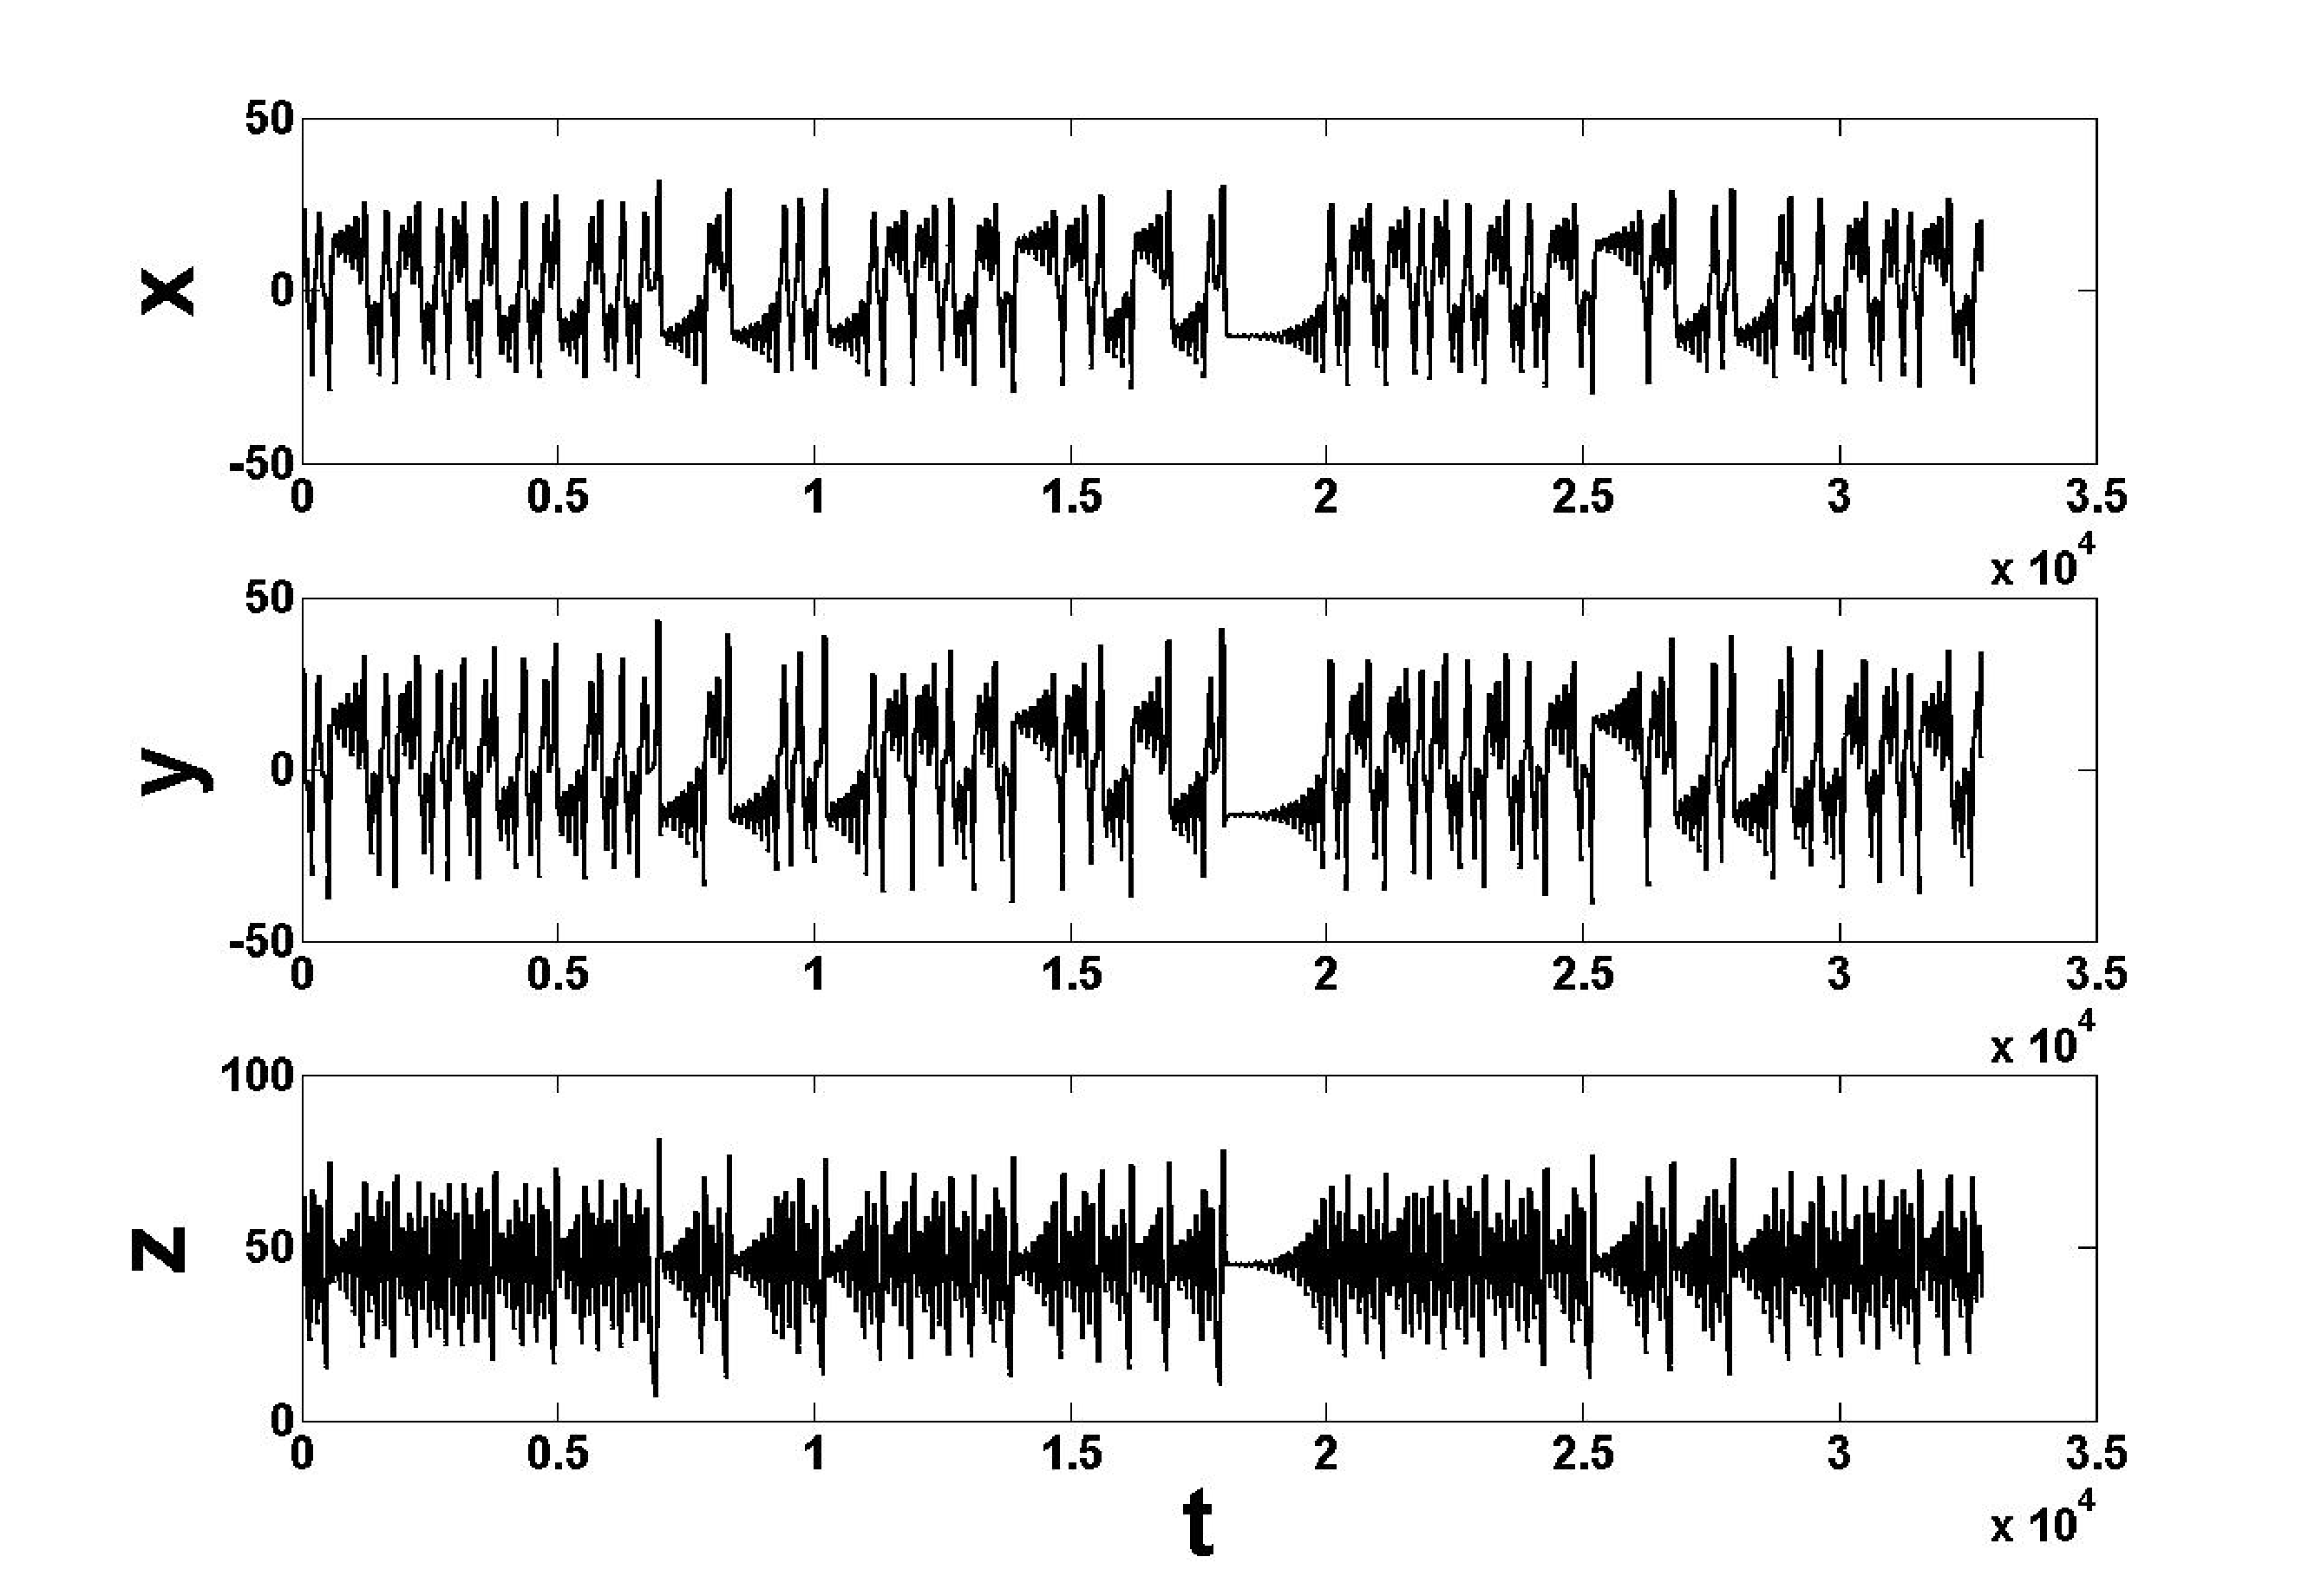
\includegraphics[width=1\columnwidth]{LorenzTiempo.pdf}\\
	\caption{Lorenz time series.}\label{fig:tiempo}
\end{figure}
%
\begin{figure}
	\centering
	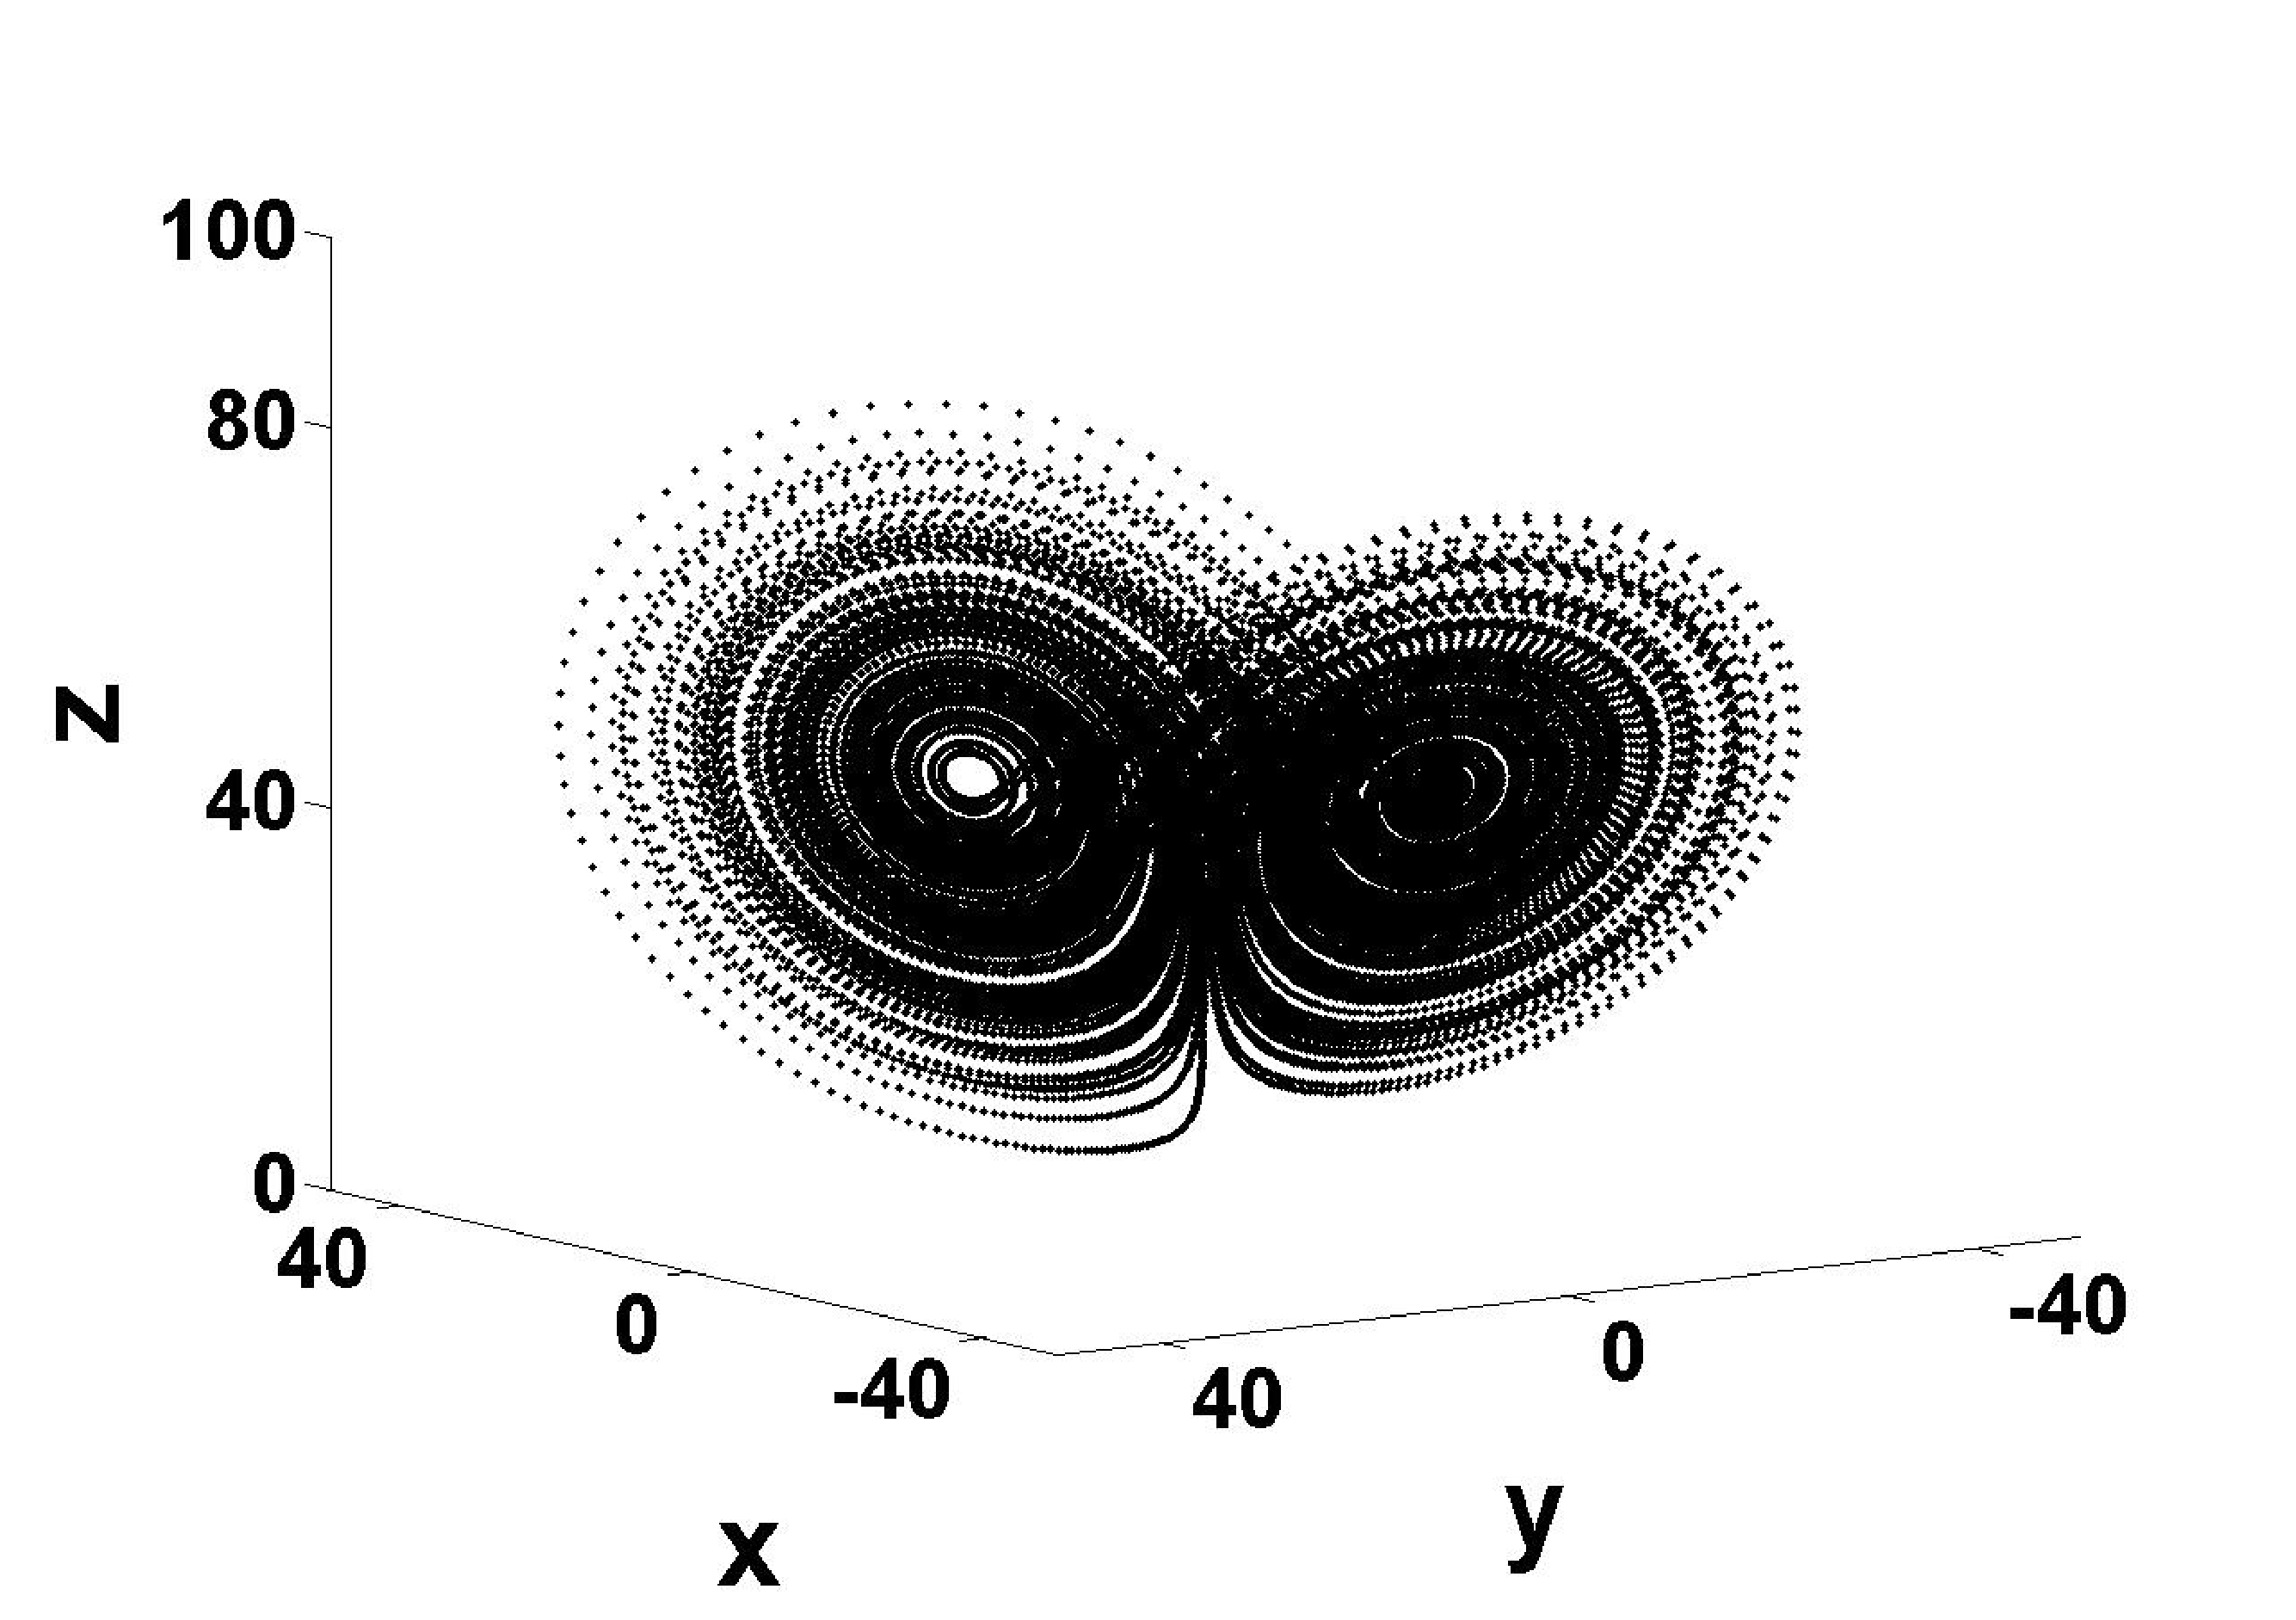
\includegraphics[width=1\columnwidth]{LorenzAtractor}\\
	\caption{Lorenz attractor.}\label{fig:atractor}
\end{figure}

El hardware requerido se muestra en la tabla \ref{tabla: Tabla1}. Aquí se muestra una comparación entre los resultados de la compilación en las tres representaciones numéricas estudiadas:
\begin{itemize}
\item \textit{aritmética de punto flotante}: los dos casos, precisión simple y doble (Flotante($32$bits) y Flotante($64$bits) respectivamente),
\item \textit{aritmética entera} (Enteros($54$bits)) y
\item \textit{aritmética de punto fijo}: los dos casos, ambos con $9$ bits de parte entera más $1$ bit de signo más los bits para la parte decimal, $22$ bits para Punto fijo($32$bits) o $54$ bits para Punto fijo($64$bits) respectivamente.
\end{itemize}
%
\begin{table*} [tb]
\begin{center}
\caption{Resultados de compilación en \textit{CYCLONE III EP3C120F780C7}.}
\begin{tabular}{|c|c|c|c|c|c|c|c|}
	\hline\hline
	                                     & Punto fijo($32$bits) & Punto fijo($64$bits) & Flotante($32$bits) & Flotante($64$bits) & Enteros($54$bits) &  \\ \hline\hline
	     Total de elementos lógicos      &       $2,392$        &       $6,104$        &      $8,176$       &      $17,532$      &      $1,297$      &  \\ \hline
	Porcentaje de elementos lógicos [\%] &        $2.00$        &        $5.12$        &       $6.86$       &      $14.72$       &      $1.08$       &  \\ \hline
	         Total de registros          &       $1,658$        &       $1,754$        &      $4,753$       &      $8,532 $      &       $159$       &  \\ \hline\hline
	       Reloj $f_{max}$ [MHz]         &       $37.82$        &       $20.51$        &       $7.48$       &       $5.42$       &      $55.38$      &  \\ \hline
	          Throughput [Mbs]           &      $1,210.24$      &       $656.32$       &      $14.96$       &      $173.44$      &    $1,772.16$     &  \\ \hline\hline
\end{tabular}\end{center}
\label{tabla:Tabla1}
\end{table*}

La implementación aritmética de enteros es la que emplea recursos mínimos y admite un $f_{max}$ más alto, la razón de esto es que las ecuaciones implementadas fueron optimizadas previamente para esta aplicación en particular.
En el caso de la representación de punto flotante, la optimización se realizó para disminuir el área, pero se pueden aplicar otras técnicas de optimización para mejorar la frecuencia o el consumo de energía \cite{Giri2012, Gokul2004}.

Para utilizar este sistema como PRNG, los datos de salida se procesan con las técnicas \textit{descarte} y \textit{concatenado}.
Ambas técnicas mantienen los bits menos significativos porque presentan el comportamiento más variable.
En el caso de la técnica de \textit{concatenado}, la parte más ruidosa de cada variable de estado se mantiene y se recombina, y se obtiene una salida de secuencia de $32$-bits en cada iteración.

Se generaron archivos de datos de análisis estocástico con $3.000.000$ palabras de $32$-bits cada uno, para $\Delta t = 2^{-n}$, con $n = 6$, $7$, $8$, $9$ y $10$.
Se calcularon las pruebas DIEHARD para todos los archivos generados.
En la tabla \ref{tabla:Tabla2} se informan algunos de los resultados más relevantes.
Definimos los valores $x_ {disc}$, ($ y_{disc}$, $z_{disc}$) como la serie temporal $x$ ($ y $, $ z $) después de aplicar la técnica de randomización por \textit{descarte}.
La variable $xyz$ es la serie de tiempo obtenida mediante la técnica de aleatorización de \textit{concatenado}.
\begin{table*} [tb]
\begin{center}
\caption{DIEHARD tests results.}
\begin{tabular}{|c|c|c|c|c|c|c|}
	\hline\hline
	                        & $\Delta t=1/2^n$ & 0,015625 & 0,0078125 & 0,00390625 & 0,001953125 & 0,0009765625 \\ \hline\hline
	   Float ($64$ bits)    &    $x_{disc}$    &    no    &    no     &     si     &     si      &      no      \\ \hline
	                        &    $y_{disc}$    &    no    &    no     &     si     &     si      &      no      \\ \hline
	                        &    $z_{disc}$    &    si    &    si     &     si     &     no      &      no      \\ \hline
	                        &      $zyx$       &    no    &    no     &     no     &     no      &      si      \\ \hline\hline
	Fixed Point ($64$ bits) &    $x_{disc}$    &    si    &    si     &     no     &     no      &      no      \\ \hline
	                        &    $y_{disc}$    &    si    &    si     &     no     &     no      &      no      \\ \hline
	                        &    $z_{disc}$    &    si    &    si     &     no     &     no      &      no      \\ \hline
	                        &      $zyx$       &    si    &    si     &     si     &     no      &      no      \\ \hline\hline
	  Integer ($54$ bits)   &    $x_{disc}$    &    si    &    si     &     no     &     no      &      no      \\ \hline
	                        &    $y_{disc}$    &    si    &    si     &     no     &     no      &      no      \\ \hline
	                        &    $z_{disc}$    &    si    &    si     &     no     &     no      &      no      \\ \hline
	                        &      $zyx$       &    si    &    si     &     si     &     si      &      si      \\ \hline
\end{tabular}\end{center}
\label{tabla:Tabla2}
\end{table*}

Esta tabla muestra que en los casos de implementaciones de enteros y punto fijo la técnica de aleatorización de \textit{descarte} funciona mejor a medida que $\Delta t$ aumenta porque, para elementos $\Delta t$ inferiores, las series temporales son más correlacionadas y esta técnica de aleatorización no los mezcla lo suficiente.
Para utilizar valores de $\Delta t$ más bajos, más bits deben descartarse para obtener buenos PRNG.
Por otro lado, la técnica de aleatorización de \textit{concatenación} funciona bien independientemente del valor de $\Delta t$ (dentro del rango analizado).

\subsection{Conclusions}
\label{sec:conclusions}

A partir de los resultados presentados aquí, es posible concluir que para obtener un PRNG, los mejores corresponden a la representación de aritmética entera tanto en hardware (recursos y frecuencia) como en propiedades estadísticas.
La técnica de aleatorización de \textit{concatenado} hace que la calidad sea independiente de $\Delta t$ para esta representación numérica.
Para la técnica de aleatorización de \textit{descarte} se obtienen buenos resultados solo para valores grandes de $\Delta t$.
Lo mismo ocurre con las implementaciones de punto fijo con ambas técnicas de aleatorización.

En términos de uso de recursos y limitaciones de frecuencia, el rendimiento en aritmética de enteros es considerablemente mejor que en punto flotante y punto fijo.
Observemos que para minimizar los recursos, se requiere un preprocesamiento del sistema caótico (escalado y polarización) para obtener divisores con una potencia de $2$, tal como se explica en la subsección \ref{sec:impleInt}.

Por otro lado, para el caso de la aritmética de punto flotante, el exponente se descarta en todas las técnicas de aleatorización utilizadas y, en consecuencia, la dinámica se ve muy perturbada por el proceso de aleatorización.
Entonces, como se muestra en la Tabla \ref{tabla: Tabla2} $\Delta t $ no es la variable relevante para predecir si un PRNG será bueno o malo.